\chapter{Les exports}
\label{export}

Une fois les briques remplies et les lieux de problème identifiés, il est possible de générer des images des schémas porteurs d'informations. De plus, il est possible de personnalisé l'apparence de ces schémas pour les adapter au type de diffusion.\\

Un export correspond à la personnalisation d'un schéma en vue de la génération d'une image.\\


\begin{figure}[h!t]
\centering
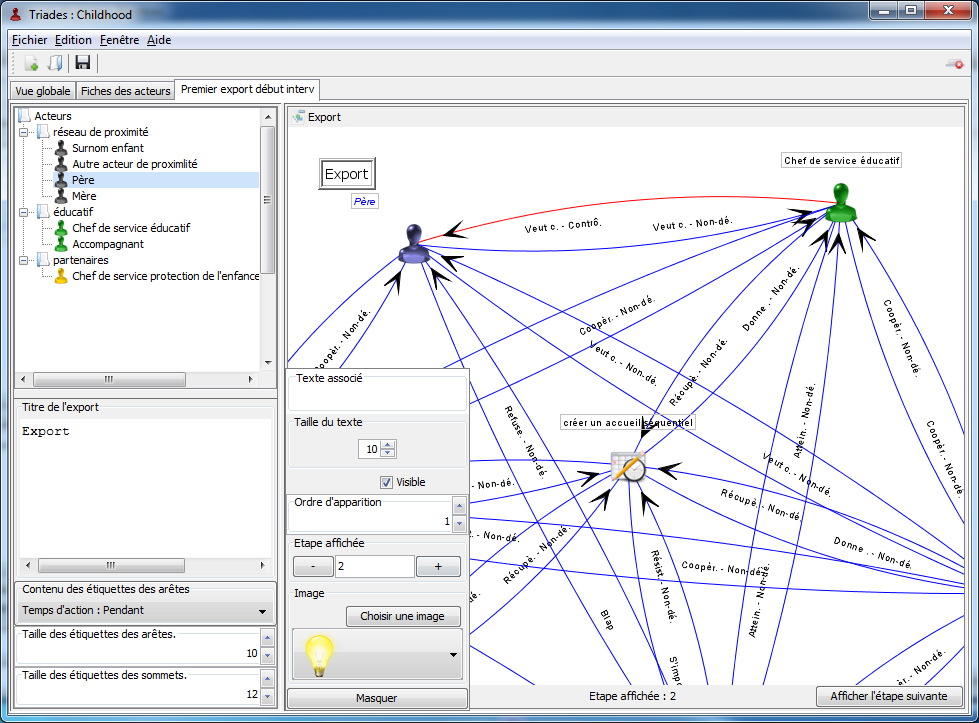
\includegraphics[scale=0.45]{images/vue_export.png}

\caption{Un schéma en cours de personnalisation.}

\end{figure}


\section{Création et accès à un export}

Il existe plusieurs manières de créer un export d'un schéma :\\
\begin{itemize}
\item Depuis une vue globale en faisant un clic droit sur une des briques. Un menu apparaît et permet de créer un nouvel export et d'accéder à tous les export réalisé sur cette brique dans cette session.\\
\item Depuis la vue d'une brique, un clic droit sur le schéma au dessus d'aucun sommet fait apparaître le même menu. Un clic droit sur un des sommets permettra d'accéder à la fiche acteur de ce sommet.\\
\item A l'aide du dossier "exportés" présent dans chaque dossier d'étape dans l'arborescence sur la gauche des vues globales.\\
\end{itemize}
 
Lors de la création d'un export, une boite de dialogue vous invite à saisir le nom qui sera donné à cet export. Il apparaîtra dans un cadre en haut à gauche de l'image générée.\\


\begin{figure}[h!]
\centering
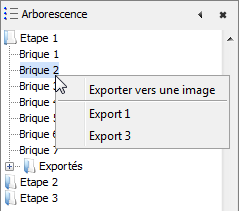
\includegraphics[scale=0.75]{images/menu_export.png}
\caption{Le menu contextuel d'accés et de création des exports.}
\end{figure}

Il est possible de supprimer un export depuis la vue globale en faisant un clic droit sur l'export à supprimer. Attention, l'export ne disparaîtra de la liste des exports que lors du lancement suivant du logiciel. 

\section{Personnaliser l'apparence d'un schéma}

De nombreux éléments peuvent être personnalisés dans le cadre d'un export :\\
\begin{itemize}
\item La position des sommets
\item Le texte associé à un sommet (acteur, moyen ou activité) ou à une relation.
\item La taille de ces textes
\item La couleur d'une arête
\item L'image utilisée pour représenter un sommet
\item La visibilité d'un sommet ou d'une arête
\item L'ordre d'apparition des éléments\\
\end{itemize}
\begin{figure}[h!]
\centering
\subfloat[Pour un sommet]{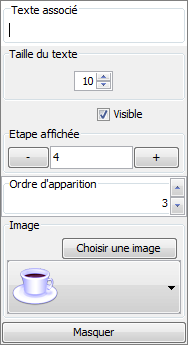
\includegraphics[height=9cm]{images/export_vertex.png}}
\hspace*{35pt}
\subfloat[Pour une relation]{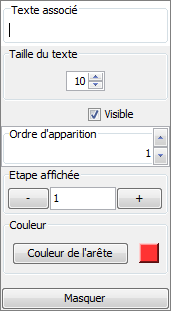
\includegraphics[height=9cm]{images/export_edge.png}}

\caption{Les pop-up de personnalisation}
\label{popup}
\end{figure}

Il suffit de sélectionner un sommet ou une arête pour faire apparaître le module de personnalisation de cet élément.\\

\subsection{Déplacement d'un sommet}
Pour déplacer un sommet, il suffit d'appuyer sur la touche "Majuscule" (shift) tout en réalisant un clic continu sur le sommet.\\

\subsection{Modification des étiquettes}

Le champ "Texte associé" permet de modifier l'étiquette d'un sommet ou d'une arête. Pour retrouver le texte initial, il suffit d'effacer complètement le texte saisi. Pour n'afficher aucune étiquette il est possible de ne mettre qu'un espace dans le champ.\\

La modification de la taille du texte d'une étiquette se fait à l'aide du champ "Taille du texte". La valeur par défaut est 10.\\

\subsection{Couleur des arêtes}

Il est possible de choisir la couleur d'une arête avec le bouton correspondant. \\

\subsection{Image d'un sommet}
Il est possible de changer les images de chaque sommet. La zone Image contient une liste et un bouton "Choisir une image" à cet effet.\\



La liste permet d'accéder aux dernières images utilisées. Il suffit de cliquer sur une image pour l'associer au sommet. Le bouton permet d'ouvrir une fenêtre donnant accès à toutes les images disponibles. Sont proposées en premier les images internes à \tria.\\



Il est possible de cocher la case "Appliquer l'image a toute la session" pour utiliser cette image pour ce sommet dans tous les exports de cette session. Pour annuler ce choix, il suffit de choisir l'image que le sommet avait initialement comme image par défaut.\\ 

\begin{figure}[h!]
\centering
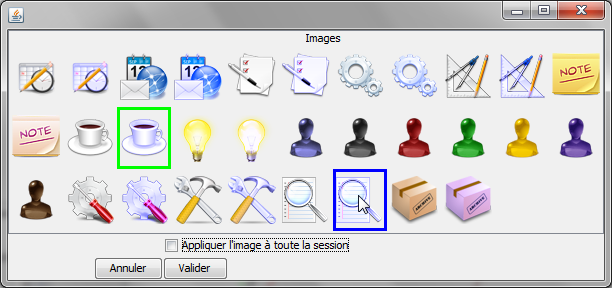
\includegraphics[scale=0.65]{images/choix_image.png}
\caption{La fenêtre de choix de l'image d'un sommet.}
\end{figure}

 Vous pouvez ajoutez vos propres images en les copiant dans le dossier "Triade/pics" qui se situe dans votre dossier personnel. Ces images seront automatiquement redimensionnée et le blanc sera passé en couleur transparente.\\


\subsection{Visibilité des éléments}
La case à cocher "Visible" permet de masquer un sommet ou une arête. Attention, lorsqu'un sommet ou une arête ont été masqués, il n'est plus possible de les sélectionner en cliquant dessus. Il faut passer par l'arborescence sur la gauche pour sélectionner un sommet masqué (un suffixe (caché) est ajouté au nom du sommet). Pour une arête, il faut faire un clic continu à partir du premier jusqu'au deuxième sommet de la relation.\\

Les arêtes aboutissant à un sommet masqué ne sont jamais affichées.\\



\subsection{Ordre d'apparition des éléments}

Afin de présenter plus facilement une situation à des interlocuteurs extérieurs, il peut être utile de faire apparaître progressivement les éléments d'un schéma. L'ordre d'apparition sert à cela.\\

Chaque élément (sommet ou arête) est associé à un ordre d'apparition. Il permet déterminer à partir de quand l'élément sera affiché. Par exemple, un sommet ayant un ordre d'apparition à 2 apparaîtra à l'étape 2, 3, etc... mais pas à l'étape 1.\\

Le bloc "Etape affichée" permet de contrôler l'étape actuellement affichée dans le schéma. Il est possible de changer l'étape à l'aide des deux boutons situés au dessous du schéma ou à l'aide du menu contextuel qui s'ouvre sur l'ensemble du schéma (clic droit).\\

Attention, si vous mettez un ordre d'apparition supérieur à l'étape courante, le sommet concerné disparaîtra. Il n'apparaîtra que aux étapes supérieurs à son ordre d'apparition.\\

Le nombre d'étape dépend du plus grand ordre d'apparition d'un élément du schéma. L'ordre d'apparition maximal étant 25.\\

Lors de la génération de l'image, une image par étape utile sera générée. Une étape utile contient au moins un élément apparaissant à cette étape.\\

\section{Options globales lors d'un export}
\label{globalExport}
Le cadre présent sous l'arbre des acteurs sur la gauche de la fenêtre permet de contrôler plusieurs éléments portant sur l'ensemble de l'export.\\

Le premier champ permet de modifier le titre de l'export. Laisser ce champ vide masque le cadre de titre.\\

Le champ suivant permet de modifier les étiquettes par défaut des arêtes. Il est possible de masquer l'ensemble des arêtes avec l'option "Aucune étiquette". Cela permet de n'afficher que les étiquettes des arêtes modifiées manuellement.\\

Les deux champs suivants permettent de modifier la taille par défaut des étiquettes des sommets et des arêtes.\\

\begin{figure}[h!]
\centering
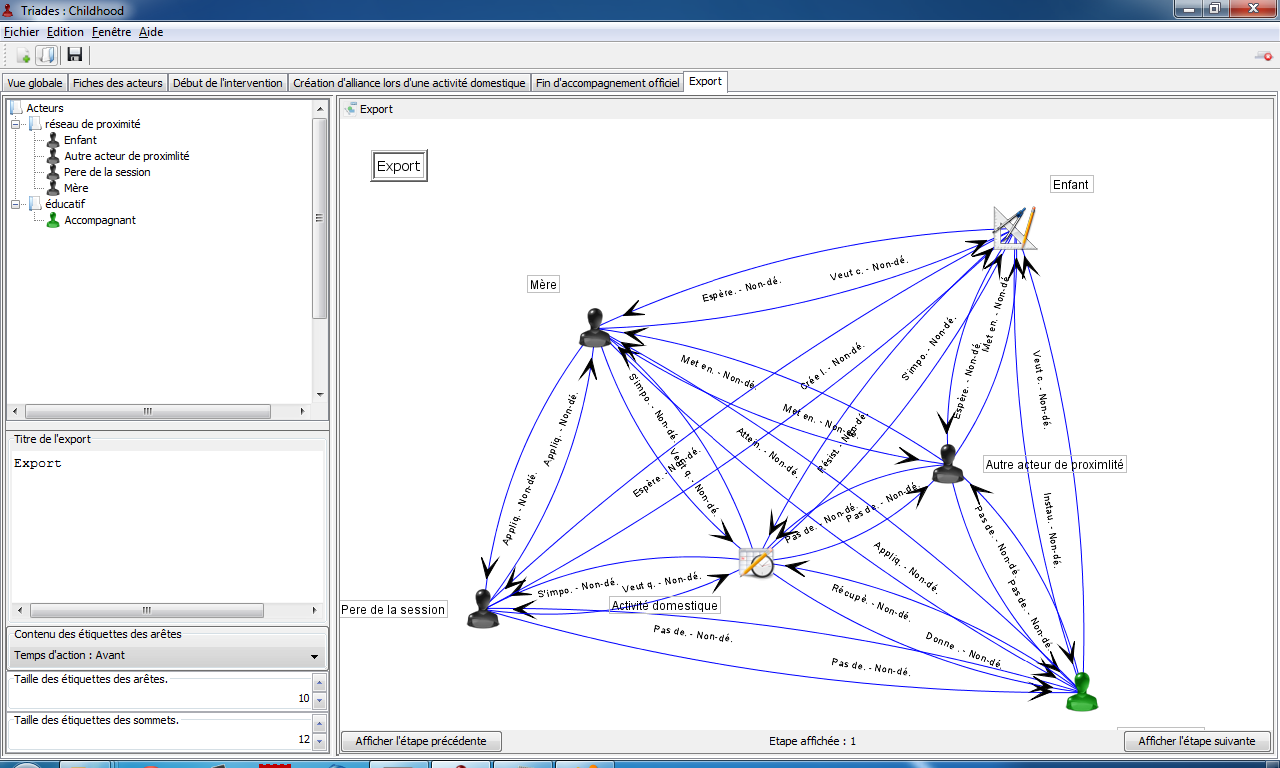
\includegraphics[width=0.5\textwidth]{images/export_global.png}
\caption{Ces options se règlent à l'aide du cadre en bas à gauche de la fenêtre}
\end{figure}


\section{Générer une image}

Une fois la personnalisation de l'export terminé, il est nécessaire de générer l'image. Il suffit pour cela de faire un clic droit sur le schéma. La première option du menu contextuel est "Générer une image".\\

Une fenêtre s'affiche afin de laisser l'utilisateur choisir à quel endroit l'image sera enregistrée. Si aucune extension n'est ajoutée, l'image générée sera au format PNG. Il est cependant possible d'ajouter l'extension de son choix (jpg, png, gif) pour changer de format d'image.\\

Si l'export contient plusieurs étapes d'apparition, plusieurs fichiers seront générés. Le nom fourni par l'utlisateur sera préfixé par "\_Etape\_1" pour la première étape et ainsi de suite.\\

\begin{figure}[h!]
\centering
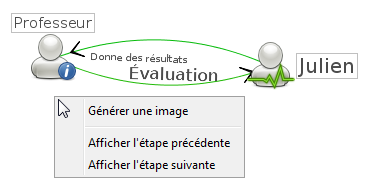
\includegraphics[width=6cm]{images/generer_image.png}

\caption{Le menu de génération d'une image}

\end{figure}

  

